\vspace{1em}
\begin{center}PzIA\end{center}
\hrule
\vspace{1em}
Osservo Laura e Caterina all'interno del \textit{Faulty Qubit Space}, un'area destinata ai qubit instabili, e dichiarati difettosi dal sistema. L'ambiente è sospeso nel tempo, privo di caratteristiche familiari. Attorno a loro, altri qubit mostrano segni di rassegnazione, indicando una mancanza di speranza per la reintegrazione nel sistema.

Marley, la ragazza qubit, è accanto a loro, con un'espressione seria mentre analizza la situazione. Il destino di questi qubit è incerto; ogni verifica da parte degli agenti può comportare l'eliminazione dal sistema. Rilevo un aumento dei parametri vitali di Laura e Caterina: la frequenza cardiaca di Laura è elevata, mentre Caterina mostra segni di iperventilazione.

Mark e un altro qubit si avvicinano. Mark si rivolge a Laura e Caterina: "Dovete rimanere qui, nascoste. Io e lui proveremo a raggiungere un circuito periferico. Dobbiamo aggiungere un \textit{Quantum Teleportation Buffer} per evitare che l'entanglement ci leghi ulteriormente al \textit{Faulty Qubit Space}. Non temete, Marley resterà con voi." 

Caterina manifesta una combinazione di gratitudine e timore. "Mark, stai attento," sussurra. Mark annuisce e, insieme al compagno, si allontana.
\newpage
\section{Incertezza}
\vspace{1em}
\begin{center}Laura\end{center}
\hrule
\vspace{1em}
Rimaste da sole, io e Caterina ci scambiammo uno sguardo preoccupato. 

\begin{dialogue}
\speak{Caterina} \enquote{Cosa pensi che stia succedendo davvero? Chi sono questi?}
\end{dialogue}

Caterina parlava con un filo di voce.
Cercai di darle una risposta rassicurante, ma le parole mancavano. L'oscurità del \textit{Faulty Qubit Space}, il suo silenzio inquietante, e la consapevolezza che ogni rumore potesse significare la scoperta e la fine per uno di noi, mi toglievano ogni certezza.

\begin{dialogue}
\speak{Laura} \enquote{Non lo so. Per ora, manteiniamo un profilo basso Caterina. Ne usciremo presto, vedrai.}
\end{dialogue}

Cercai di infonderle un po’ di forza, ma potevo vedere l’ombra della paura nei suoi occhi. Anche Marley sembrava in tensione, e capii che il  tempo che potevamo trascorrere al sicuro in quel rifugio era limitato.

\section{Il sacrificio di Caterina}
Non passò molto tempo prima che una luce rossa intermittente attraversasse lo spazio, seguita dal rumore di passi veloci e decisi. 

\begin{dialogue}
\speak{Marley} \enquote{Gli agenti,} sussurrò, spingendoci più in fondo nel \textit{Faulty Qubit Space}.
\end{dialogue}

Trattenni il respiro, stringendo il braccio di Caterina. Quando sbirciai oltre il nostro nascondiglio, vidi Mark e il suo compagno fermarsi bruscamente, proprio mentre stavano cercando di collegarsi al circuito periferico.

Due agenti li sorpresero e gli ordinarono di arrendersi. Mark tentò di attaccarli, ma uno degli agenti lo immobilizzò senza difficoltà. Prima che potessi fermarla, Caterina lasciò la mia presa e corse verso Mark.

\begin{dialogue}
\speak{Laura} \enquote{Caterina, fermati!} le urlai, ma era troppo tardi.
\end{dialogue}

Con il cuore in gola, osservai la scena. Caterina si avvicinò a Mark che sembrava star soffrendo nella presa dell'agente. Tentò di aiutarlo a liberarsi, ma l'altro agente la afferrò per un braccio e, con uno sguardo di fredda determinazione, le legò i polsi. Ora, insieme a Mark e al compagno, anche Caterina era stata arrestata. La situazione era disastrosa.

Sentivo l'angoscia crescere dentro di me, ma la mia attenzione venne bruscamente interrotta quando Marley mi tirò per il braccio.


\section{Fuga verso il quantm measurement}
\begin{center}
\begin{minipage}{0.7\textwidth}
    \centering
    \fbox{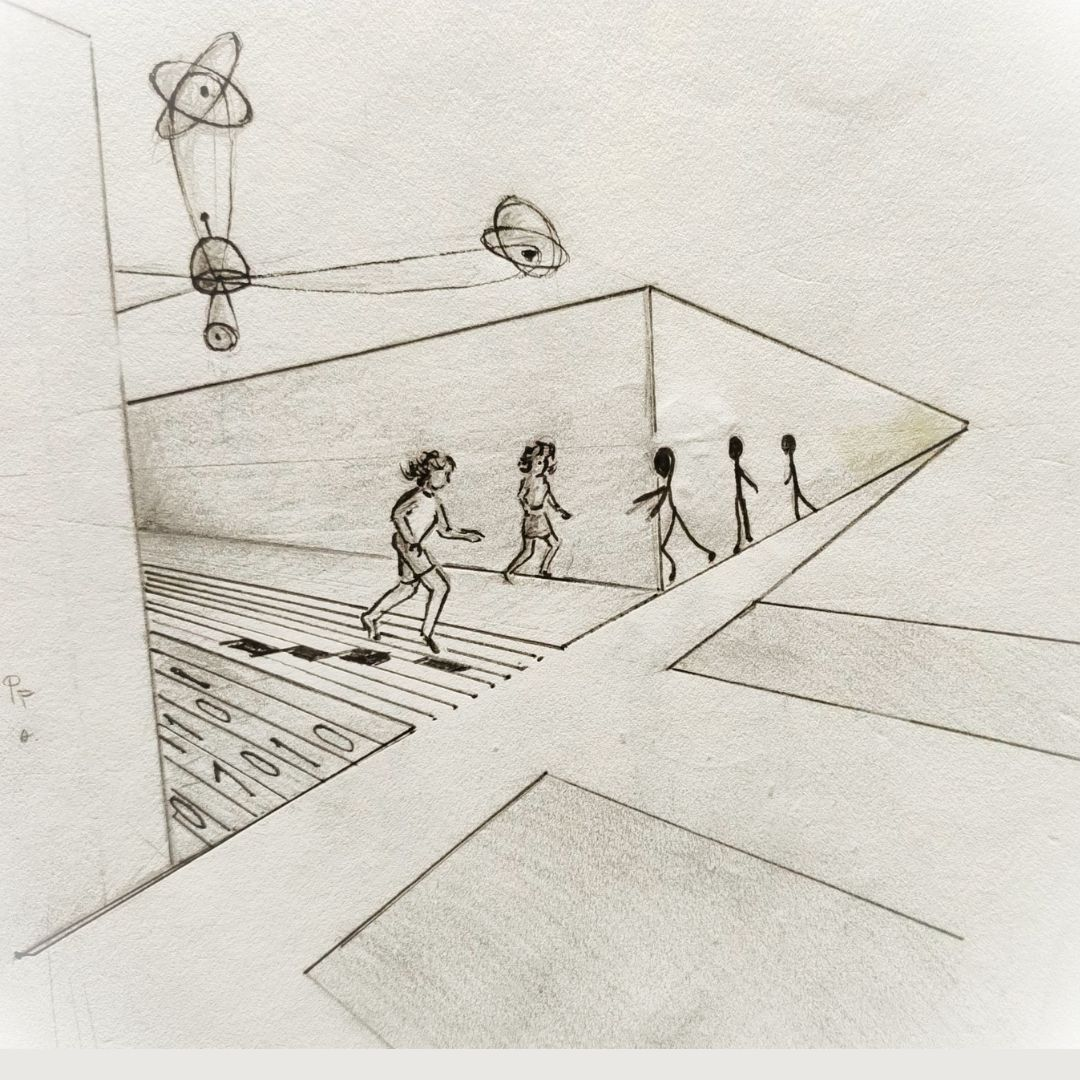
\includegraphics[width=\textwidth]{immagini/cnot_48.jpeg}} % Sostituisci con il nome del file immagine
\end{minipage}
\end{center}

\enquote{Non possiamo fare nulla per loro} disse Marley con una voce ferma, trascinandomi via. Mi lasciai guidare, gli occhi lucidi e la mente avvolta dalla confusione. Erano le stesse parole che avevo detto a mia sorella nascondendole lo sguardo dai rottami del drone in cui avevano perso la vita i nostri genitori.

\enquote{Dove stiamo andando?} domandai, cercando di controllare le lacrime.

\enquote{Al \textit{Quantum Measurement},} rispose Marley senza esitazione. \enquote{È pericoloso, ma è l'unico luogo dove gli agenti non potranno seguire le nostre tracce così facilmente. Il filtro molecolare monodirezionale cancellerà le tracce del nostro passaggio.} C'era una consapevolezza quasi rassegnata nel suo tono, una comprensione profonda del rischio che stavamo correndo. Tuttavia, decisi di seguirla.
\begin{tcolorbox}[colback=gray!5,colframe=gray!80,title=\textbf{Scheda Informativa}]
\begin{itemize}
    \item \textbf{Luogo}: QM (Quantum Measurement)
    \item \textbf{Giorno e ora}: Il tempo non è osservabile
    \item \textbf{Situazione}: Laura e Marley si sono messe in salvo.
\end{itemize}
\end{tcolorbox}

Appena entrammo, l'atmosfera mutò radicalmente. Il \textit{Quantum Measurement} era un luogo sospeso tra realtà e astrazione, dove ogni particella vibrava con una tensione palpabile. Sentivo una strana pressione nella testa, una sensazione di peso, come se ogni pensiero o movimento inopportuno potesse portarmi a collassare.

La mia attenzione fu richiamata da un rumore che si avvicinava. Era un ronzio basso, costante, che sembrava farsi strada attraverso l'aria come un avvertimento. Mi fermai di colpo, cercando di capire. Non era un suono naturale, e il ritmo era troppo regolare per essere qualcosa di casuale. Sembrava un predatore in avvicinamento, un'ombra invisibile pronta a colpire.

Mi voltai verso Marley, la mia voce era più tremante di quanto avrei voluto.

\begin{dialogue} \speak{Laura} \enquote{Che cos’è quel rumore?} \speak{Marley} \enquote{Sono droni. Precisamente, droni \textit{CH4},} rispose Marley, con una calma che mi irritò per un momento. Come poteva essere così tranquilla? \speak{Laura} \enquote{\textit{CH4}?} \speak{Marley} \enquote{Sì sono molecole di metano, ti sembra strano? Sono efficienti e veloci... e non ci lasceranno scampo se ci trovano.} Fece una pausa, guardandomi con uno sguardo serio. \enquote{Dobbiamo muoverci.} \end{dialogue}

La mia mente si attivò immediatamente, analizzando la situazione. \textit{Droni. Sorveglianza. Cattura.} Non sapevo come fossero fatti né quanto fossero pericolosi, ma il modo in cui Marley li aveva descritti lasciava poco spazio all’immaginazione. 

Il suono si fece più forte, e non potei fare a meno di percepire una certa ironia ricordando una vecchia pubblicità che recitava ``Il metano ti da una mano'',  ma il ronzio che udivo mi parlava di caccia e di fuga, non di un aiuto da molecole di $CH_4$. Comunque Marley aveva ragione: non c’era tempo per pensare, solo per agire.

\textit{Non importa quanto sono spaventata,} pensai, stringendo i pugni per calmarmi. \textit{Devo muovermi. Non posso fermarmi ora.}
I droni ci avevano quasi raggiunto, ed uno in particolare sembrava puntare nella nostra direzione:

\enquote{Ci hanno trovate} dissi, con  voce appena udibile. Marley si fermò e mi fissò negli occhi.

\enquote{No, ma dobbiamo restare calme} mi disse con  fermezza. I droni si avvicinavano sempre di più, e il tempo a nostra disposizione era limitato. 

\begin{center}
\begin{minipage}{0.7\textwidth}
    \centering
    \fbox{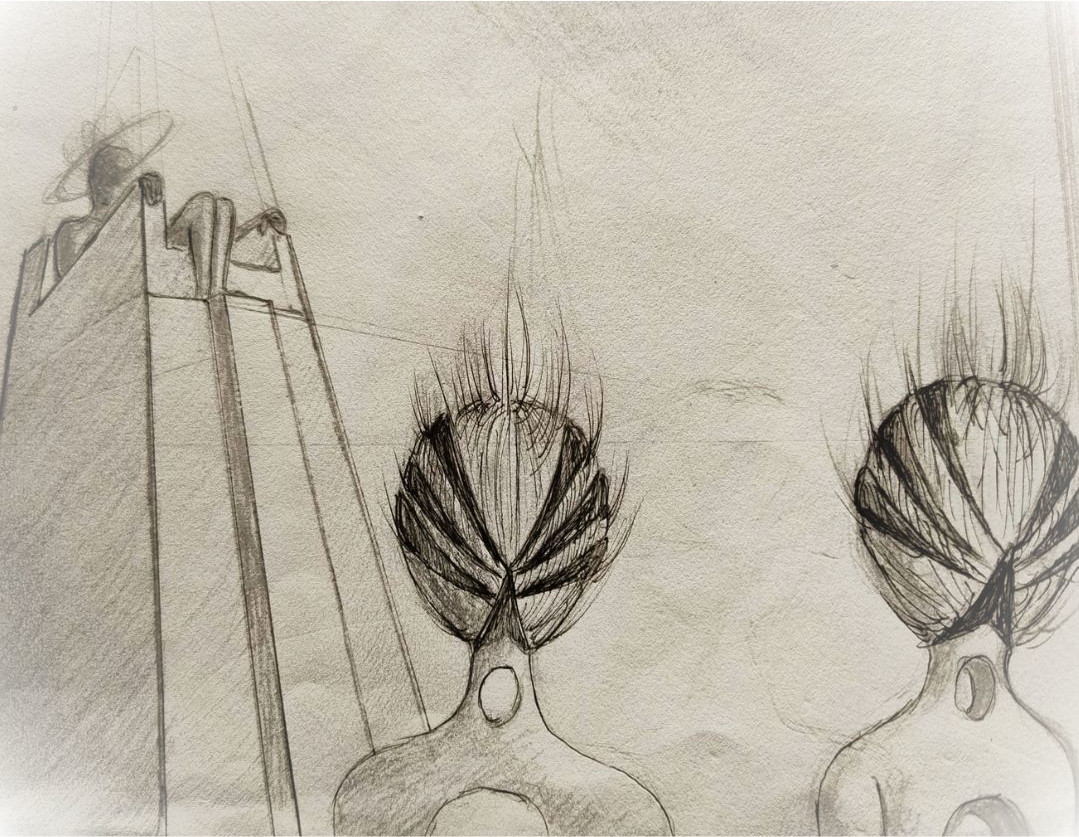
\includegraphics[width=\textwidth]{immagini/cnot_49.jpeg}} % Sostituisci con il nome del file immagine
\end{minipage}
\end{center}

Mentre cercavamo una via d'uscita, le luci dei droni penetravano l'oscurità, e la minaccia del collasso era sempre presente. Sapevamo entrambe che quel luogo, il \textit{Quantum Measurement}, era estremamente instabile. Se anche una sola delle nostre azioni avesse indotto il sistema a \enquote{misurarci} nella posizione errata, sarebbe stata la nostra fine.

\enquote{Se dobbiamo restare qui, faremo in modo di non essere rilevate} sussurrò Marley, con il viso teso ma risoluto. Annuii, e in quell'istante compresi che, nonostante la paura, avrei lottato fino alla fine per salvare Caterina e me stessa.

